\documentclass[11pt,a4paper]{article}
\usepackage[T1]{fontenc}
\usepackage[margin=2.3cm]{geometry}
\usepackage{amsmath,amssymb}
\usepackage{graphicx}
\usepackage[dvipsnames]{xcolor}
\usepackage{enumitem}
\usepackage[colorlinks=true,linkcolor=blue,urlcolor=blue]{hyperref}
\setlength{\parskip}{0.6em}
\setlength{\parindent}{0pt}
\begin{document}

\begin{center}{\LARGE\bfseries openelevator}\\[0.4em]{\large Design a lift ride that is quick and comfortable, in three sessions.}\\[0.2em]\small PAN IIT OSS explainer \textbullet{} middle school to higher secondary (levels 2-4)\end{center}

\section*{Why this exists}
Every lift ride is a balance between speed and comfort. This explainer shows the mathematics behind it: a speed-time graph, Newton's second law for a car on a rope with a counterweight, and a time-stepping simulation you can check by hand.

\section*{The end goal}
Design an elevator ride that is quick and comfortable (counterweight, motor, jerk). The end goal is to design a lift ride that is quick and comfortable, choosing the motion profile and motor with a counterweight and jerk limit. This is an educational model only; real lifts are designed and certified to safety standards by qualified engineers.

\section*{How the three sessions build up}
\begin{enumerate}[nosep]
\item \textbf{Session 1: A lift going up and down: speed, graphs and why you feel heavier} (Level 1, conceptual interactive model, 60 min).
\item \textbf{Session 2: Motion profiles, comfort limits and motor power} (Level 2, mathematical engineering model, 75 min).
\item \textbf{Session 3: Simulating the whole lift: torque limit, comfort and energy} (Level 3, simulation and validation, 90 min).
\end{enumerate}

\section{Session 1: A lift going up and down: speed, graphs and why you feel heavier}

\subsection*{A. Real-world problem}
You step into a lift and, as it starts to rise, the floor seems to push harder on your feet. When it slows near the top you feel a little lighter. Nothing about you has changed, and gravity has not changed either. What has? And how can a designer make a ride quick without making the push on your feet unpleasant?

\subsection*{B. Concept and theory}
A lift ride is simplest to describe with a speed-time graph. The lift speeds up at a constant acceleration a until it reaches the top speed v, travels at v, then slows down at the same rate. The graph is a trapezoid. The slope of the graph is the acceleration and the area under it is the distance. Speeding up to v takes v / a seconds and covers v\textasciicircum{}2 / (2 a) metres, slowing down is the same, so a ride of distance d takes d / v + v / a seconds as long as d is at least v\textasciicircum{}2 / a. If the distance is shorter, the lift never reaches v. You feel the force of the floor on your feet, the apparent weight N. Newton's second law for you says net force = mass x acceleration, and the net force is N upward minus your weight m g downward, so N = m (g + a). When the lift accelerates upward (speeding up while going up, or slowing down while going down) a is positive and you feel heavier. When the acceleration points down you feel lighter. At constant speed a = 0 and N = m g. Only the acceleration matters, never the speed.

\begin{itemize}[nosep]
\item d: distance travelled (m)
\item v: top (cruise) speed (m/s)
\item a: acceleration of the lift, upward positive (m/s\textasciicircum{}2)
\item m: mass of the person (kg)
\item g: gravitational acceleration, 9.81 (m/s\textasciicircum{}2)
\item N: force of the floor on the person (apparent weight) (N)
\item T: total ride time (s)
\end{itemize}

\begin{equation*}
T=\frac{d}{v}+\frac{v}{a}\qquad (d\ge v^2/a)
\end{equation*}

\begin{equation*}
d_{\text{accelerate}}=\frac{v^2}{2a},\qquad t_{\text{accelerate}}=\frac{v}{a}
\end{equation*}

\begin{equation*}
N-mg=ma\;\Rightarrow\;N=m\,(g+a)
\end{equation*}

\begin{center}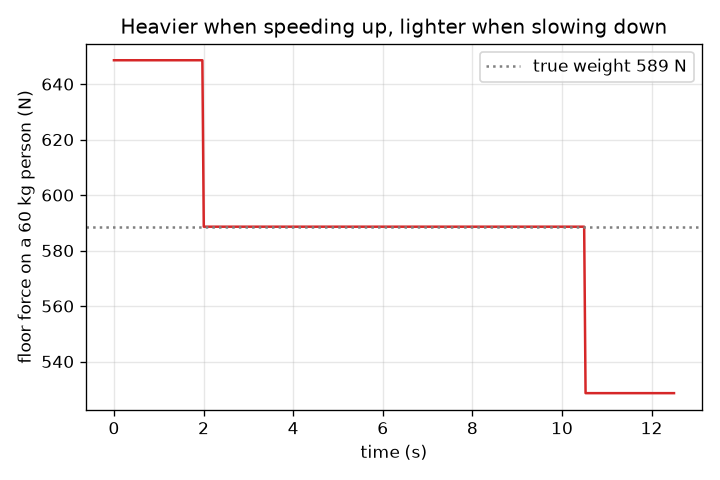
\includegraphics[width=0.85\linewidth]{figures/s01_apparent_weight.png}\\\small Floor force on a 60 kg person: heavier while speeding up, lighter while slowing down.\end{center}

\subsection*{E. Worked example}
A 60 kg person is in a lift that speeds up upward at 1.0 m/s\textasciicircum{}2. What force does the floor exert, and how does it compare with the person's weight at rest?
\begin{enumerate}[nosep]
\item Weight at rest: m g = 60 * 9.81 = 588.6 N.
\item While speeding up: N = m (g + a) = 60 * (9.81 + 1.0) = 60 * 10.81 = 648.6 N.
\item Ratio: 648.6 / 588.6 = 1.10, so the person feels 10 percent heavier.
\item Slowing down at the same rate (a = -1.0): N = 60 * 8.81 = 528.6 N, about 10 percent lighter.
\end{enumerate}
\textbf{Answer.} N = 648.6 N while speeding up (588.6 N at rest, 528.6 N while slowing down).

\subsection*{F. Questions}
\begin{enumerate}[nosep]
\item \textbf{Conceptual.} A lift is moving downward at a steady speed and then begins to slow down to stop at the ground floor. Do you feel heavier, lighter or the same? Explain without using the word speed.
\item \textbf{Numerical.} A 75 kg person stands in a lift that speeds up upward at 1.5 m/s\textasciicircum{}2. Find the floor force and the percentage change from the person's weight at rest.
\item \textbf{Graph and simulation interpretation.} On the speed-time graph of the 21 m ride (top speed 2 m/s, rise over 2 s, flat for 8.5 s), what is the acceleration and how can you check that the distance is 21 m?
\item \textbf{Design and optimisation challenge.} Design: the 21 m ride must take less than 11 s and the floor force must stay within 15 percent of the person's weight (a \textless{}= 1.47 m/s\textasciicircum{}2). Choose a and v, check d \textgreater{}= v\textasciicircum{}2 / a, and give the ride time. Why not simply choose a very large v?
\end{enumerate}

\section{Session 2: Motion profiles, comfort limits and motor power}

\subsection*{A. Real-world problem}
Two floors are 3.5 m apart. Session 1 said the ride is quick if the acceleration is large, but a lift that jumps from rest to 1 m/s\textasciicircum{}2 in an instant feels like a jolt even if the acceleration is small. What really makes a ride comfortable? And how big must the motor be, given that a counterweight balances most of the car? Finally, can the same recipe run a 20-floor express?

\subsection*{B. Concept and theory}
Jerk is the rate of change of acceleration, j = da/dt, measured in m/s\textasciicircum{}3. A trapezoid profile changes acceleration instantly (infinite jerk on paper), which passengers feel as a jolt at the start and the end of each speed change. An S-curve profile ramps the acceleration up and down at a limited jerk j. It has up to seven phases: jerk +j, constant acceleration, jerk -j, cruise, jerk -j, constant braking, jerk +j. Typical design values for passenger comfort are an acceleration of about 1 to 1.5 m/s\textasciicircum{}2 and a jerk of about 1 to 2 m/s\textasciicircum{}3; we use 1.0 m/s\textasciicircum{}2 and 1.5 m/s\textasciicircum{}3 as assumed values, not as a standard. To reach speed v the acceleration phase lasts Ta = v / a + a / j if v \textgreater{}= a\textasciicircum{}2 / j (the acceleration reaches its limit), and Ta = 2 sqrt(v / j) otherwise. Speeding up and slowing down together cover v Ta, so if d \textgreater{}= v Ta the ride takes T = d / v + Ta. For a short ride the cruise speed is lowered until v Ta = d; when the acceleration reaches its limit this gives v\textasciicircum{}2 + (a\textasciicircum{}2 / j) v - a d = 0. The car, passengers and a counterweight hang on one rope over the motor sheave, so the motor only has to carry the unbalanced weight (m\_car + m\_load - m\_cw) g, plus a force M a to accelerate the total moving mass M = m\_car + m\_load + m\_cw. At constant speed the motor input power is P = (m\_car + m\_load - m\_cw) g v / eta. A negative value means the load drives the motor.

\begin{itemize}[nosep]
\item j: jerk, rate of change of acceleration (m/s\textasciicircum{}3)
\item a: acceleration limit (m/s\textasciicircum{}2)
\item v: cruise speed (maximum speed) (m/s)
\item Ta: time to speed up from rest to v (s)
\item d: distance of the ride (m)
\item T: travel time (s)
\item m\_car, m\_load, m\_cw: car, passenger and counterweight masses (kg)
\item eta: motor and gear efficiency (0 to 1) (no unit)
\item P: motor input power (W)
\end{itemize}

\begin{equation*}
T_{\text{trap}}=\frac{d}{v}+\frac{v}{a}\quad(d\ge v^2/a),\qquad T_{\text{trap}}=2\sqrt{d/a}\quad(d<v^2/a)
\end{equation*}

\begin{equation*}
T_a=\frac{v}{a}+\frac{a}{j}\quad(v\ge a^2/j),\qquad T=\frac{d}{v}+T_a\quad(d\ge vT_a)
\end{equation*}

\begin{equation*}
v^2+\frac{a^2}{j}v-ad=0\quad\text{(short ride, cruise speed set by the distance)}
\end{equation*}

\begin{equation*}
P=\frac{(m_{\text{car}}+m_{\text{load}}-m_{\text{cw}})\,g\,v}{\eta}
\end{equation*}

\begin{equation*}
F=(m_{\text{car}}+m_{\text{load}}-m_{\text{cw}})\,g+(m_{\text{car}}+m_{\text{load}}+m_{\text{cw}})\,a
\end{equation*}

\begin{center}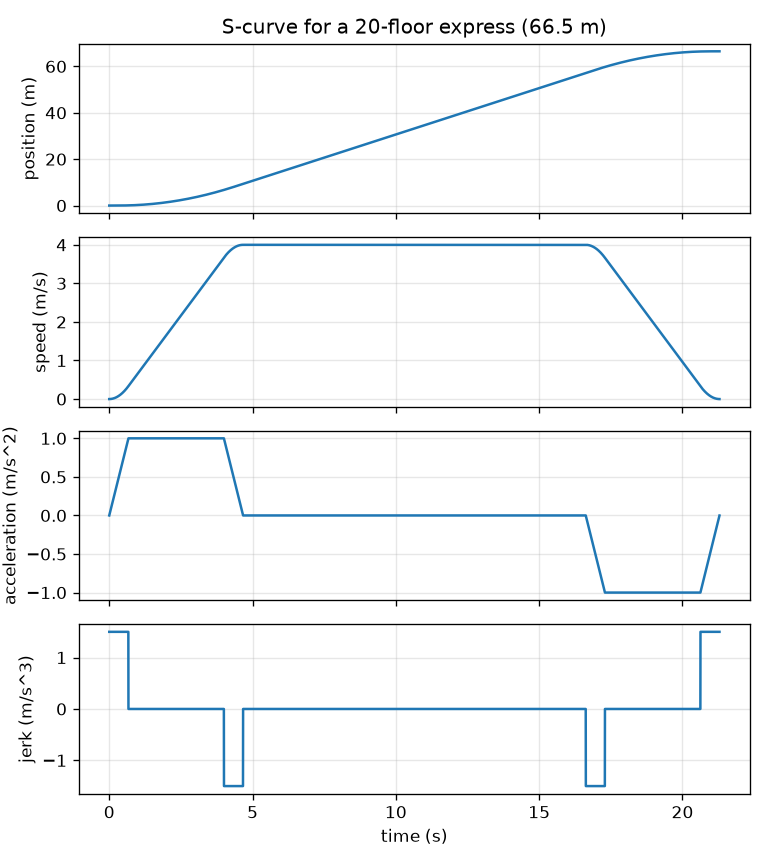
\includegraphics[width=0.85\linewidth]{figures/s02_scurve_profile.png}\\\small An S-curve ride for 66.5 m: position, speed, acceleration and jerk against time.\end{center}

\subsection*{E. Worked example}
Two floors are 3.5 m apart. With a maximum speed of 2.5 m/s, acceleration limit 1.0 m/s\textasciicircum{}2 and jerk limit 1.5 m/s\textasciicircum{}3, find the S-curve travel time and the cruise speed reached. Then find the motor power at that speed for a full car (1000 kg car, 800 kg load, 1360 kg counterweight, eta = 0.85).
\begin{enumerate}[nosep]
\item Check the full speed first: reaching 2.5 m/s needs Ta = 2.5 / 1.0 + 1.0 / 1.5 = 3.167 s, and v Ta = 7.9 m, much more than 3.5 m. The lift cannot reach 2.5 m/s.
\item Assume the acceleration reaches 1.0 m/s\textasciicircum{}2. Then v\textasciicircum{}2 + (a\textasciicircum{}2 / j) v - a d = 0 becomes v\textasciicircum{}2 + 0.6667 v - 3.5 = 0.
\item v = (-0.6667 + sqrt(0.4444 + 14)) / 2 = (-0.6667 + 3.8006) / 2 = 1.567 m/s. This is above a\textasciicircum{}2 / j = 0.667 m/s, so the assumption holds.
\item Ta = 1.567 / 1.0 + 1.0 / 1.5 = 2.234 s and, with no cruise, T = 2 Ta = 4.467 s. The trapezoid with the same acceleration needs 2 sqrt(3.5) = 3.74 s.
\item Unbalanced mass = 1000 + 800 - 1360 = 440 kg. P = 440 * 9.81 * 1.567 / 0.85 = 7956 W, about 7.96 kW.
\end{enumerate}
\textbf{Answer.} The S-curve ride takes 4.47 s with a cruise speed of 1.57 m/s (the trapezoid takes 3.74 s); the cruise power for a full car going up is about 7.96 kW.

\subsection*{F. Questions}
\begin{enumerate}[nosep]
\item \textbf{Conceptual.} A trapezoid ride and an S-curve ride have the same peak acceleration. Why does the S-curve feel better, and what does it cost?
\item \textbf{Numerical.} For a 14 m ride with maximum speed 2.0 m/s, a = 1.0 m/s\textasciicircum{}2 and j = 1.5 m/s\textasciicircum{}3, find the S-curve travel time. Compare with the trapezoid.
\item \textbf{Graph and simulation interpretation.} On the time-versus-distance figure, why does the gap between the two curves stay constant for long rides but the S-curve is relatively slower for short rides?
\item \textbf{Design and optimisation challenge.} Design: (1) What is the fastest ride between two floors 3.5 m apart if the comfort limits are a \textless{}= 1.5 m/s\textasciicircum{}2 and j \textless{}= 2.0 m/s\textasciicircum{}3? (2) For the 20-floor express (66.5 m) with a top speed of 4 m/s and the original limits (1.0 and 1.5), find the ride time and the cruise motor power for a full car. State one trade-off.
\end{enumerate}

\section{Session 3: Simulating the whole lift: torque limit, comfort and energy}

\subsection*{A. Real-world problem}
Session 2 gave a clean plan. A real lift does not follow its plan exactly: its motor force takes a moment to build up, it has a limit, and a full car going up needs far more force than an empty one. If the motor is too small the ride falls behind its plan and the passengers feel it. How can we test this before building anything, and how do we know the simulation can be trusted? And what happens to the energy when a heavy car goes down?

\subsection*{B. Concept and theory}
The car, passengers and counterweight move together, so Newton's second law for the whole system is M a = F - (m\_car + m\_load - m\_cw) g, which gives F = (m\_car + m\_load - m\_cw) g + M a, with M = m\_car + m\_load + m\_cw. The motor force F cannot exceed a limit F\_max (its torque limit divided by the sheave radius), and it builds up with a time constant tau: dF/dt = (F\_cmd - F) / tau. A controller asks for the force that would follow the plan, a\_cmd = a\_plan + kv (v\_plan - v) + kp (x\_plan - x). We step the equations forward in time with dt = 1 ms. The simulated acceleration is a = (F - unbalance) / M and the jerk is its time derivative. Comfort is judged by the peak \textbar{}a\textbar{} and peak \textbar{}jerk\textbar{} actually produced; we score it as the larger of peak a / 1.2 and peak jerk / 2.5 (assumed limits, a score of at most 1 is comfortable). We validate in two ways. First, with no saturation the simulated ride time must match the exact formula T = d / v + v / a + a / j. Second, since the speed starts and ends at zero, the net mechanical work of the motor must equal the change of potential energy of the unbalanced mass, integral of F v dt = (m\_car + m\_load - m\_cw) g d. When this work is negative (heavy car going down, or light car going up) the motor is driven and can feed energy back, at efficiency eta.

\begin{itemize}[nosep]
\item F: motor force on the rope (up positive) (N)
\item F\_max: motor force limit (torque limit / sheave radius) (N)
\item M: total moving mass m\_car + m\_load + m\_cw (kg)
\item tau: time constant of the motor force (s)
\item kp, kv: controller gains (position and speed) (1/s\textasciicircum{}2 and 1/s)
\item dt: time step (s)
\item peak a, peak jerk: largest acceleration and jerk felt (m/s\textasciicircum{}2 and m/s\textasciicircum{}3)
\item E: energy drawn from or fed back to the grid (J)
\item eta: efficiency of motor and drive (no unit)
\end{itemize}

\begin{equation*}
F=(m_{\text{car}}+m_{\text{load}}-m_{\text{cw}})\,g+M\,a,\qquad M=m_{\text{car}}+m_{\text{load}}+m_{\text{cw}}
\end{equation*}

\begin{equation*}
\tau\,\dot F=F_{\text{cmd}}-F,\qquad F_{\text{cmd}}=\mathrm{clip}\big(\text{unbalance}+M\,a_{\text{cmd}},\,-F_{\max},\,F_{\max}\big)
\end{equation*}

\begin{equation*}
a_{\text{cmd}}=a_{\text{plan}}+k_v\,(v_{\text{plan}}-v)+k_p\,(x_{\text{plan}}-x)
\end{equation*}

\begin{equation*}
\int F\,v\,dt=(m_{\text{car}}+m_{\text{load}}-m_{\text{cw}})\,g\,d\qquad(\text{speed is zero at both ends})
\end{equation*}

\begin{equation*}
P_{\text{el}}=\frac{F v}{\eta}\ (Fv\ge 0),\qquad P_{\text{el}}=\eta\,F v\ (Fv<0,\ \text{fed back})
\end{equation*}

\begin{center}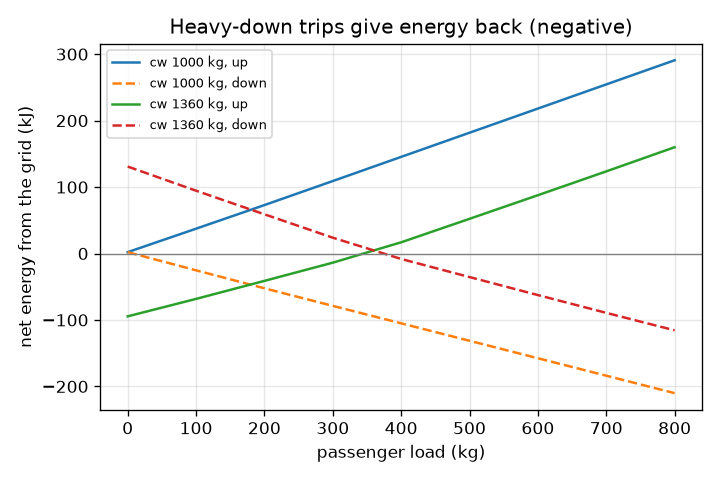
\includegraphics[width=0.85\linewidth]{figures/s03_energy_vs_load.png}\\\small Net energy from the grid against load: heavy cars going down feed energy back.\end{center}

\subsection*{E. Worked example}
A half-loaded car (400 kg of passengers) rides 31.5 m up with maximum speed 2.5 m/s, acceleration 1.0 m/s\textasciicircum{}2 and jerk limit 1.5 m/s\textasciicircum{}3. (1) What travel time does the formula give and what does the simulation give? (2) What mechanical work should the motor do, and does the simulation agree? (3) A full car (800 kg) goes down the same 31.5 m: how much energy is fed back?
\begin{enumerate}[nosep]
\item Formula: T = d / v + v / a + a / j = 31.5 / 2.5 + 2.5 / 1.0 + 1.0 / 1.5 = 12.6 + 2.5 + 0.667 = 15.77 s. The simulation gives 15.77 s (15.770 s), a difference of about 3 ms.
\item Unbalanced mass = 1000 + 400 - 1360 = 40 kg. Work = 40 * 9.81 * 31.5 = 12 360 J, about 12.4 kJ. The simulated integral of F v dt is 12.35 kJ, within 1 percent.
\item Full car going down: unbalanced mass = 1000 + 800 - 1360 = 440 kg, so the work is -440 * 9.81 * 31.5 = -136.0 kJ. The motor is driven during the whole ride, so the grid supplies nothing.
\item Energy fed back = eta * 136.0 kJ = 0.85 * 136.0 = 115.6 kJ, which is what the simulation reports (115.6 kJ).
\item Comfort check: the simulated peak acceleration is 1.04 m/s\textasciicircum{}2 and the peak jerk is 2.13 m/s\textasciicircum{}3, both within the limits (score 0.87).
\end{enumerate}
\textbf{Answer.} T = 15.77 s (formula and simulation agree within 3 ms), motor work 12.4 kJ going up, and a full car going down feeds back 115.6 kJ.

\subsection*{F. Questions}
\begin{enumerate}[nosep]
\item \textbf{Conceptual.} The trapezoid plan never asks for more than 1.0 m/s\textasciicircum{}2, yet the simulated trapezoid ride peaks at 1.41 m/s\textasciicircum{}2 with a very large jerk. Why?
\item \textbf{Numerical.} A car carrying 200 kg goes up 31.5 m. Use the energy balance to find the mechanical work, and say whether the grid draws or receives energy over the whole ride.
\item \textbf{Graph and simulation interpretation.} On the energy-against-load figure, why does the 'up' curve for the 1360 kg counterweight cross zero at a load of 360 kg, and what does a lighter counterweight do?
\item \textbf{Design and optimisation challenge.} Design: for the 10-storey building (31.5 m), the car has 1000 kg, the rated load is 800 kg, the counterweight is 1360 kg. Choose the smallest motor force limit from 6000, 7000, 7500, 8000 and 9000 N and the profile, so that the comfort score is below 1 and the motor never saturates. Give the peak electrical power and one trade-off.
\end{enumerate}

\section{Real-world mini-project}
\textbf{Choose the motor and the profile for a 10-storey building.} A building has 10 storeys with 3.5 m between floors, so the longest ride is 9 floors = 31.5 m. The lift has an empty car of 1000 kg, a rated load of 800 kg and a counterweight of 1360 kg. Passengers must feel a peak acceleration of at most 1.2 m/s\textasciicircum{}2 and a peak jerk of at most 2.5 m/s\textasciicircum{}3 (assumed comfort limits), the ride must follow its plan (travel time within 0.02 s of the formula) and the motor force limit must never be reached. Candidate motor force limits are 6000, 7000, 7500, 8000 and 9000 N. Use \texttt{plan}, \texttt{simulate} and \texttt{comfort\_score} from Session 3 to test the worst cases, a full car going up and an empty car going down, with the trapezoid and with the S-curve (maximum speed 2.5 m/s, acceleration 1.0 m/s\textasciicircum{}2, jerk 1.5 m/s\textasciicircum{}3).

\section{The path ahead}
\begin{enumerate}[nosep]
\item \textbf{Session 4: Cleaner jerk: feed-forward the force lag.} A controller that anticipates the motor lag, so that the jerk the passengers feel stays close to the jerk of the plan.
\item \textbf{Session 5: Fastest ride inside the comfort box.} A search that picks the plan with the shortest travel time whose simulated ride stays inside a peak acceleration of 1.2 m/s\textasciicircum{}2 and a peak jerk of 2.5 m/s\textasciicircum{}3.
\item \textbf{Session 6: A day of traffic: energy over many trips.} An estimator of the energy used in a day of 200 trips with random loads and directions, compared with the counterweight mass.
\item \textbf{Session 7: A stretchy rope: car vibration.} A two-mass model (car and sheave) joined by a spring that represents the rope stretch.
\item \textbf{Session 8: Two lifts, one lobby: group control.} A simulation of two lifts serving a 10-floor building with random calls.
\end{enumerate}

\section{Answers and hints}

\subsection*{Session 1}
\begin{enumerate}[nosep]
\item \textbf{Conceptual.} Hint: Slowing down while moving down means the velocity changes toward up. Which way does the acceleration point? Solution: You feel heavier. The velocity is downward and shrinking, so the change of velocity (the acceleration) points upward. With a upward and positive, N = m (g + a) is larger than m g. What matters is the direction of the acceleration, not the direction of the motion.
\item \textbf{Numerical.} Hint: N = m (g + a) with g = 9.81 m/s\textasciicircum{}2. Solution: N = 75 * (9.81 + 1.5) = 75 * 11.31 = 848.25 N, about 848 N. Weight at rest = 75 * 9.81 = 735.75 N. Change = 848.25 / 735.75 = 1.153, so 15.3 percent heavier. Unit check: kg * m/s\textasciicircum{}2 = N.
\item \textbf{Graph and simulation interpretation.} Hint: Slope = rise over run. Area = two triangles and a rectangle. Solution: Slope of the rising part = (2 - 0) / 2 = 1.0 m/s\textasciicircum{}2. Area: two triangles of 0.5 * 2 * 2 = 2 m each (4 m) plus a rectangle 2 m/s * 8.5 s = 17 m, total 21 m, which matches the distance.
\item \textbf{Design and optimisation challenge.} Hint: Try a = 1.4 m/s\textasciicircum{}2 and a few values of v in T = d / v + v / a. Solution: Take a = 1.4 m/s\textasciicircum{}2 (a/g = 0.143, so 14.3 percent). With v = 3 m/s: v\textasciicircum{}2 / a = 6.4 m, which is less than 21 m, so the lift reaches full speed. T = 21 / 3 + 3 / 1.4 = 7.0 + 2.14 = 9.14 s, below 11 s. A very large v is not free: the lift needs a stronger motor, more shaft height to slow down safely, and passengers dislike very high speed. With a = 1.4 the time stays under 11 s only for v above about 2.2 m/s, so a v of 2.5 to 4 m/s is a sensible range. Assumptions: constant acceleration, no jerk limit (Session 2 adds it).
\end{enumerate}

\subsection*{Session 2}
\begin{enumerate}[nosep]
\item \textbf{Conceptual.} Hint: Compare how quickly the acceleration changes at the start of the ride, and compare the travel times. Solution: In the trapezoid the acceleration jumps from 0 to its full value at once, so the jerk is infinite on paper and passengers feel a jolt; in the S-curve the acceleration is ramped at a limited jerk, so the force on the body changes gradually. The cost is time: the ramps mean the average acceleration is lower. For long rides the extra time is a / j (0.67 s for a = 1.0 and j = 1.5); for short rides the lift may also never reach its top speed.
\item \textbf{Numerical.} Hint: Ta = v / a + a / j, then check d \textgreater{}= v Ta. Solution: Ta = 2.0 / 1.0 + 1.0 / 1.5 = 2.667 s and v Ta = 5.33 m, which is less than 14 m, so the lift cruises. T = d / v + Ta = 14 / 2.0 + 2.667 = 9.667 s. Trapezoid: T = 14 / 2.0 + 2.0 / 1.0 = 9.0 s. The S-curve is 0.667 s slower (a / j).
\item \textbf{Graph and simulation interpretation.} Hint: For long rides T = d / v + something that does not depend on d. Solution: For long rides both times are d / v plus a fixed amount (v / a for the trapezoid, v / a + a / j for the S-curve), so their difference is a / j = 0.667 s whatever d is. For short rides the lift never reaches its top speed and the jerk ramps take a larger share of a short trip, so the gap in relative terms is larger (0.73 s on a 3.5 m ride, 19 percent longer than the trapezoid).
\item \textbf{Design and optimisation challenge.} Hint: Use v\textasciicircum{}2 + (a\textasciicircum{}2 / j) v - a d = 0 for part (1), and T = d / v + v / a + a / j for part (2). Solution: (1) v\textasciicircum{}2 + (2.25 / 2.0) v - 1.5 * 3.5 = 0, i.e. v\textasciicircum{}2 + 1.125 v - 5.25 = 0, so v = (-1.125 + sqrt(1.2656 + 21)) / 2 = 1.797 m/s (above a\textasciicircum{}2 / j = 1.125 m/s, so a reaches its limit). Ta = 1.797 / 1.5 + 1.5 / 2.0 = 1.948 s and T = 2 Ta = 3.90 s, against 4.47 s with the gentler limits. (2) T = 66.5 / 4 + 4 / 1.0 + 1.0 / 1.5 = 16.625 + 4 + 0.667 = 21.29 s; cruise power = 440 * 9.81 * 4 / 0.85 = 20.3 kW. Trade-off: raising the limits saves time (0.57 s on the short ride) but passengers feel more; a higher top speed saves time on the express but needs more power and a longer slowing distance.
\end{enumerate}

\subsection*{Session 3}
\begin{enumerate}[nosep]
\item \textbf{Conceptual.} Hint: Think about what a sudden step in the plan does to a motor force that takes time to build up and a controller that corrects errors. Solution: The plan jumps in acceleration, but the motor force can only build up with the time constant tau = 0.05 s, so the lift lags behind the plan at first. The feedback controller then asks for extra force to catch up, and the force overshoots, so the acceleration peaks above the plan. The sudden change also forces a large rate of change of force, which is the jerk (about a / tau). The S-curve asks for gradual changes that the motor can follow, so it hardly overshoots.
\item \textbf{Numerical.} Hint: Unbalanced mass = 1000 + 200 - 1360. Work = unbalanced mass * g * d. Solution: Unbalanced mass = 1000 + 200 - 1360 = -160 kg, so the work is -160 * 9.81 * 31.5 = -49.4 kJ: the counterweight is heavier and pulls the car up, so the motor is driven. Over the ride the motor still draws a little energy while accelerating and gives back more while braking: in the simulation the grid supplies 3.1 kJ and receives 44.2 kJ, a net of -41.2 kJ (energy fed back). Check: 0.85 * 49.4 = 42.0 kJ, close to 41.2 kJ, because the acceleration phases add small losses in both directions.
\item \textbf{Graph and simulation interpretation.} Hint: When is the unbalanced mass zero? Solution: The net mechanical work is (1000 + load - cw) g d, zero when load = cw - 1000 = 360 kg (the car is perfectly balanced), apart from the small losses of accelerating. Below that load the car going up is lighter than the counterweight and energy is fed back, above it the motor draws energy. A lighter counterweight (1000 kg) moves the zero to a load of 0 kg, so every load costs more going up and gives back more going down.
\item \textbf{Design and optimisation challenge.} Hint: Hand estimate: F needed is about the unbalanced weight plus M a at full load. Then use simulate() on a full car going up and an empty car going down. Solution: Hand estimate: full car, F = 440 * 9.81 + 3160 * 1.0 = 4316 + 3160 = 7476 N, so about 7.5 kN is needed; the simulation peak is 7608 N because the controller overshoots slightly. The 6000 N and 7000 N motors saturate, and the ride has peak accelerations above 3 m/s\textasciicircum{}2 (score above 19), while 7500 N follows the plan (score 0.87). The trapezoid has a score of 11.1 even with the 7500 N motor and 8.8 with 9000 N, so it never passes. Choose the S-curve with a 7500 N motor (a margin would suggest 8000 N). The peak electrical power of the full-car ride up is about 19.2 kW, so the drive should be rated above that. Trade-off: a bigger motor costs more and handles loads better, a smaller jerk limit gives a gentler ride but a longer travel time.
\end{enumerate}

\section{How to join}
Read \texttt{CONTRIBUTING.md} in the repository, then pick an issue labelled \texttt{good first issue}. Repository: \url{https://github.com/KrunalPanchal1995/openelevator}

\end{document}
